\section{Durchführung}
\label{sec:Durchführung}

\subsubsection{Untersuchung der Amplitude und Berechnung des Dämpfungwiderstandes}

Zur Untersuchung der Zeitanhängigkeit der Amplitude und zur Berechnung des Dämpfungwiderstandes
wird ein gedämpfter Schwingkreis gemäß Abbildung \ref{fig:gsk2} aufgebaut. Dieser wird mit einem
Nadelimpulsgenerator so angeregt, dass zwischen zwei Impulsen die Amplitude um den Faktor drei 
bis acht abgenommen hat. Weiterhin soll der kleinere der beiden Festwiderstände verwendet werden
und um Abweichungen der Messungen durch andere Bauteile zu vermeiden, wird ein hochohmiger 
Tastkopf mit $R_i = 10\, \si{\mega\ohm}$ verwendet.

\begin{figure}[H]
  \centering
  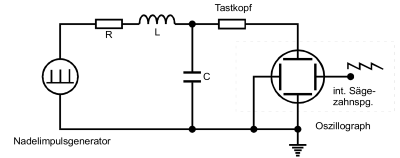
\includegraphics{content/aufgabeA.png}
  \caption{Schaltskizze eines gedämpften Schwingkreises zur Berechnung des Dämpfungwiderstandes und zur Untersuchung der Zeitanhängigkeit der Amplitude}
  \label{fig:gsk2}
\end{figure}

Das Bild des Spannungsverlaufs auf dem Oszilloskop soll aufgenommen werden und anschließend soll
zur Bestimmung des Dämpfungwiderstandes $R_{eff}$, sowie der Abklingdauer $T_ex$ die Kondensatorspannung
$U_C$ gegen die Zeit aufgetragen werden. Der errechnete Wert von $R_{eff}$ soll anschließend mit dem
tatsächlichen Wert $R$ aus der Schaltung verglichen werden.


